\documentclass{scrartcl}

\usepackage[T1]{fontenc}
\usepackage[utf8]{inputenc}

\title{Mobile Dev Week 2 Lab}
\author{Daniel Coady (102084174)}
\date{23/08/2019}

\usepackage{graphicx}

\begin{document}

\maketitle

\section*{Conversion App}

\begin{figure}[h]
    \centering
    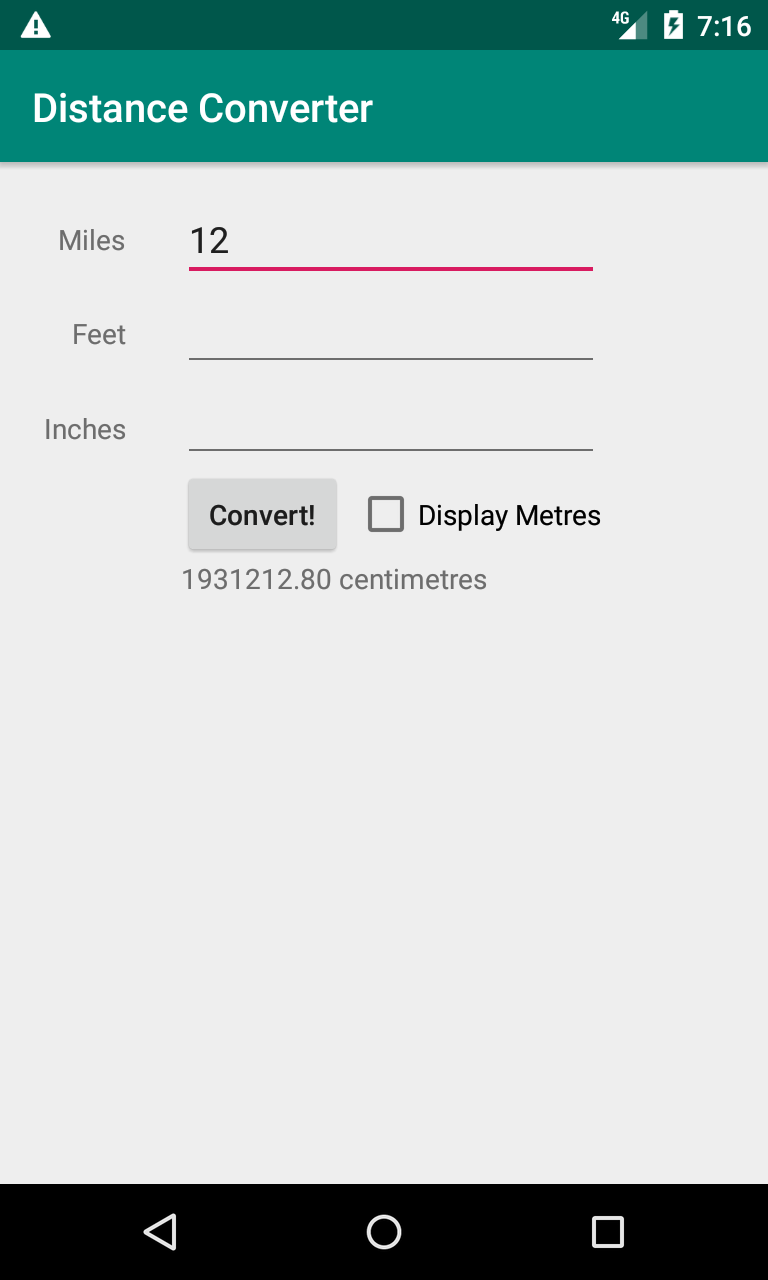
\includegraphics[scale=0.2]{images/portrait.png}
    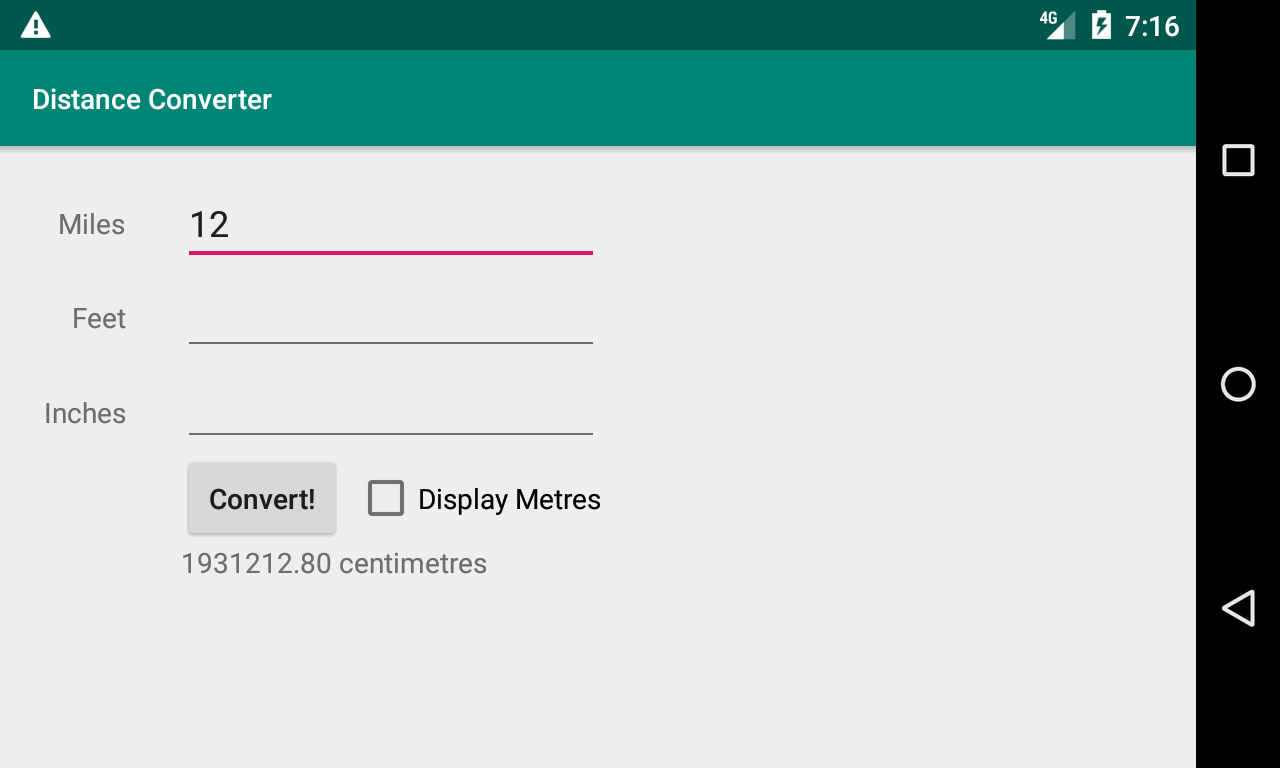
\includegraphics[scale=0.2]{images/landscape.png}
    \caption{Conversion app in portrait and landscape}
\end{figure}

\pagebreak

\section*{Localisation}

\begin{figure}[h]
    \centering
    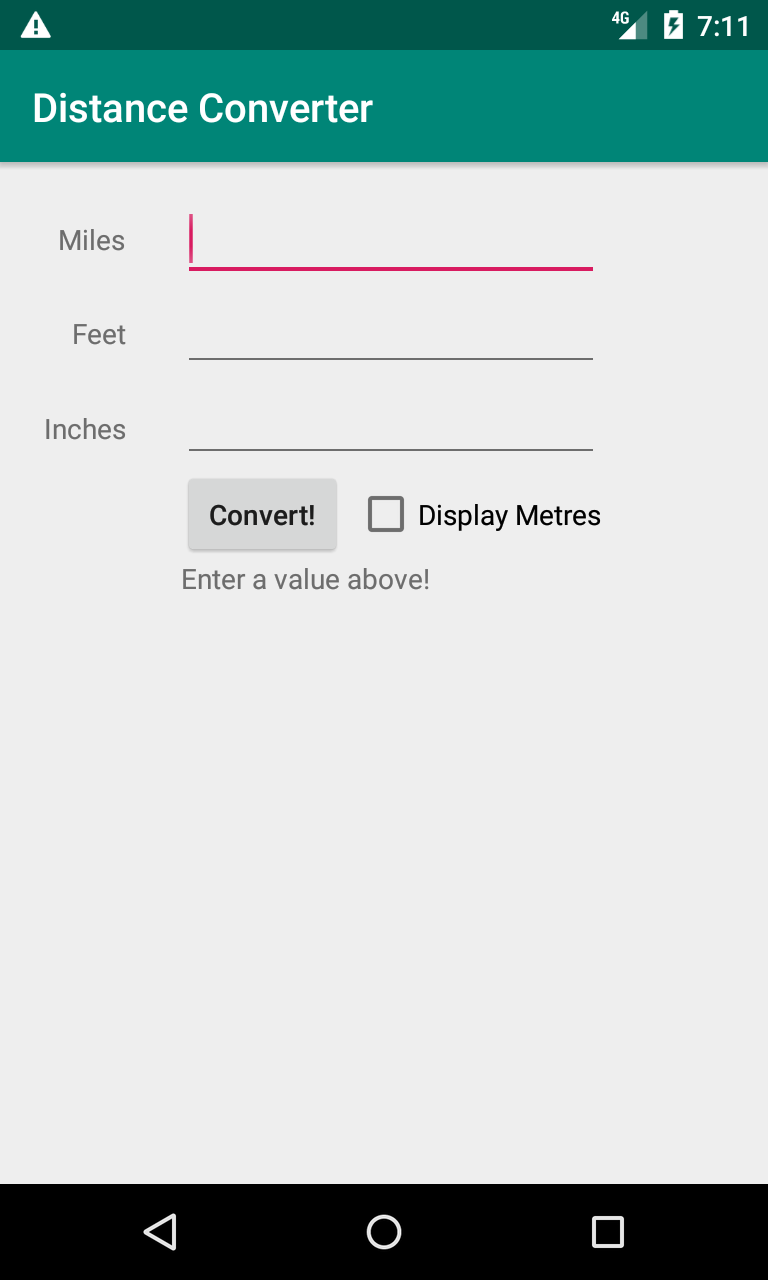
\includegraphics[scale=0.2]{images/english.png}
    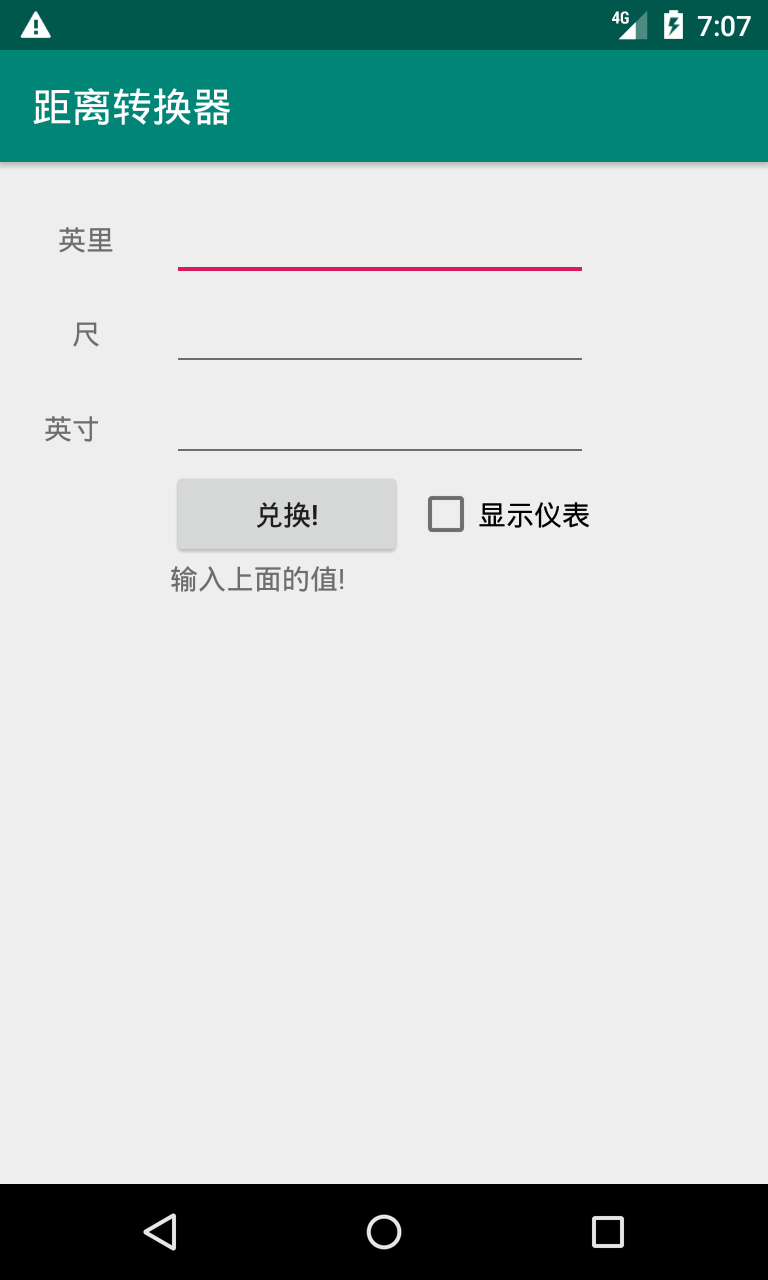
\includegraphics[scale=0.2]{images/chinese.png}
    \caption{Conversion app in English and Chinese}
\end{figure}

In Android development, when you design an interface it's important that you use as many references
to resources in the app as possible so that you can more easily perform localisation tasks. This is
because you can create sets of resources for different locales, and these resources will be switched
out when the locale of the device is changed. In this instance, we have two string files set up for
our interface that contains all the strings that the user would see when looking at the application.
One of these files acts as the default which contains everything in English. When we want to display
a string to the screen we reference from within the resources, showing the corresponding string.
In our second file of strings (which is for Chinese locales in this example) we have all of the exact
same string names, but different strings that have been translated into Chinese. Now when the
application detects the Chinese locale it switches to using the Chinese resources for the app. Since
we told the application to display strings from the resources file, it will now start pulling strings
from our Chinese strings file and display those instead. This system allows for us to create localisations
for our applications easily.

\end{document}
